\newpage
\clearpage
\onecolumn
\appendix

\section{Appendix}


\section{A \quad Metrics} \label{app:exp:metric}
\subsection{A.1 \quad Total Task Latency}

We define \textbf{Total Task Latency} as the total time taken by the multi-agent system to complete a full episode of the task, from initial context routing to final memory update. It serves as a key metric to evaluate the runtime efficiency of different routing strategies (e.g., Full-Context, Static Routing, RCR-Router).

We consider two latency formulations:

\paragraph{Wall-clock latency.} This measures the actual elapsed time during task execution:
\begin{equation}
\text{TotalTaskLatency} = T_{\text{end}} - T_{\text{start}}
\end{equation}
where $T_{\text{start}}$ is the timestamp when the task begins (e.g., user query issued or memory initialized), and $T_{\text{end}}$ is the time when the task completes (e.g., final recommendation returned).

\paragraph{Iterative agent latency (parallel).} When multiple agents operate concurrently per routing iteration, total latency is the sum of the maximum agent time per iteration:
\begin{equation}
\text{TotalTaskLatency} = \sum_{k=1}^{K} \max_{i \in \mathcal{A}} \text{Latency}_{i}^{(k)}
\end{equation}
where $K$ is the number of routing-feedback iterations, $\mathcal{A}$ is the set of agents, and $\text{Latency}_{i}^{(k)}$ is the time taken by agent $i$ in iteration $k$.

\paragraph{Sequential agent latency (serial).} In systems without concurrency, total latency is computed as:
\begin{equation}
\text{TotalTaskLatency} = \sum_{k=1}^{K} \sum_{i \in \mathcal{A}} \text{Latency}_{i}^{(k)}
\end{equation}

Unless otherwise stated, we adopt the parallel agent latency model to reflect the practical deployment scenarios of multi-agent LLM systems with concurrent execution support.


\subsection{A.2 \quad Per-round Runtime}

To better understand the temporal behavior of our system, we analyze the \textbf{per-round runtime}---the amount of time consumed during each routing-feedback iteration $t \in \{1, 2, \dots, K\}$. This metric provides insight into how the iterative routing mechanism scales with the number of reasoning rounds and the complexity of the memory store.

Let $\text{Runtime}^{(t)}$ denote the total runtime of all agents in iteration $t$. We define:
\begin{equation}
\text{Runtime}^{(t)} = \sum_{i \in \mathcal{A}} \text{Latency}_{i}^{(t)}
\end{equation}
where $\mathcal{A}$ is the set of participating agents (e.g., Planner, Searcher, Recommender), and $\text{Latency}_{i}^{(t)}$ is the time consumed by agent $i$ during iteration $t$.

We report per-round runtime statistics in Table~\ref{tab:main_results}, including average, minimum, and maximum values across test episodes. Our analysis shows that:
\begin{itemize}
    \item Runtime generally increases in early rounds due to richer memory and larger context sizes.
    \item Later iterations tend to stabilize or reduce latency as context becomes more focused.
    \item RCR-Router introduces moderate overhead per round due to token-budgeted filtering and importance scoring.
\end{itemize}
Despite the additional routing overhead, RCR-Router remains within practical runtime bounds and offers substantial gains in task success rates.

%\subsection{A.3  \quad Task Success Rate}

%We report \textbf{Task Success Rate} as the primary metric for evaluating multi-agent task completion across different routing strategies. A task is considered successful if the final agent outputs align with the ground-truth objective specified by the benchmark (e.g., identifying the correct product in WebShop or answering the question in HotPotQA).

%Formally, let $N$ denote the total number of evaluation episodes. Define a success indicator function $\mathbb{I}_{\text{success}}^{(n)}$ for episode $n$ such that:
%\begin{equation}
%\text{TaskSuccessRate} = \frac{1}{N} \sum_{n=1}^{N} \mathbb{I}_{\text{success}}^{(n)} \times 100\%
%\end{equation}

%We evaluate success rate under various routing settings:
%\begin{itemize}
%    \item \textbf{Full-Context Routing}: All agents access the entire shared memory in every round.
%    \item \textbf{Static Routing}: Agents receive fixed, handcrafted contexts.
%    \item \textbf{RCR-Router (Ours)}: Agents are provided with semantically routed contexts under token budget constraints.
%\end{itemize}

%As shown in Table~\ref{tab:main_results}, our RCR-Router achieves consistently higher success rates across multiple benchmarks while maintaining better efficiency. Notably, the iterative routing design contributes to improved contextual alignment and decision accuracy.

\subsection{A.3  \quad Total Token Consumption (K)}

We report \textbf{Total Token Consumption} as a key efficiency metric that reflects the aggregate number of tokens used in LLM prompts across all agents and routing iterations. This directly impacts both computational cost and real-world deployment feasibility for multi-agent LLM systems.

Formally, let $\mathcal{A}$ denote the set of agents, and $K$ the number of routing-feedback iterations. Then the total token usage is computed as:
\begin{equation}
\text{TotalTokenConsumption} = \sum_{t=1}^{K} \sum_{i \in \mathcal{A}} \text{TokensUsed}_{i}^{(t)}
\end{equation}
where $\text{TokensUsed}_{i}^{(t)}$ denotes the number of prompt and response tokens associated with agent $i$ in iteration $t$.

We compare token consumption across three routing strategies:
\begin{itemize}
    \item \textbf{Full-Context Routing}: All agents receive the full memory $M_t$ each round, resulting in maximal token usage.
    \item \textbf{Static Routing}: Each agent receives a fixed handcrafted subset of memory (e.g., by role tags), offering limited savings.
    \item \textbf{RCR-Router (Ours)}: Agents receive semantically filtered and token-budgeted contexts, significantly reducing token usage without degrading performance.
\end{itemize}

%As shown in Table~\ref{tab:token_consumption}, RCR-Router achieves a strong trade-off: it maintains high task success rates while reducing token usage compared to Full-Context Routing. In many cases, over 30\% token savings are observed relative to naive full-context baselines.

\subsection*{A.4  \quad Answer Quality Score}

We design an automatic scoring mechanism to evaluate the quality of generated outputs in multi-agent LLM systems. The process is implemented via a prompt-based evaluation using DeepSeek~\cite{liu2024deepseek,lu2024deepseek} LLM, which returns a JSON object containing a score and justification. The evaluation prompt and scoring logic are as follows:

\subsection*{Prompt Construction}

Given a user query $Q$ and a model-generated answer $A$, we construct a system prompt $P$ as:

\begin{quote}
You are an expert judge. Your task is to evaluate how well the answer responds to the user's query.

User Query: \textbackslash n
\{\{Q\}\}

Answer: \textbackslash n
\{\{A\}\}

Please provide a JSON object with the following format:
\{"score": (1 to 5), "justification": "a short explanation of the score"\}

\end{quote}

\subsection*{Scoring Algorithm}

\begin{enumerate}
    \item \textbf{Input:} A user query $Q$ and the corresponding generated answer $A$.
    \item \textbf{Build Prompt $P$} using a standardized scoring instruction template.
    \item \textbf{Send $P$ to an LLM Scoring Engine} (e.g., DeepSeek, GPT-4) via API call:
    \[
        \texttt{output} \leftarrow \texttt{llm\_query\_api}(P)
    \]
    \item \textbf{Parse Score:} Convert the LLM output into a JSON object and extract the numerical score:
    \[
        \texttt{score} \leftarrow \texttt{json.loads(output)["score"]}
    \]
    \item \textbf{Return:} A quality score in the range $[1, 5]$, with optional justification text.
\end{enumerate}

\subsection*{Remarks}
This scoring framework is model-agnostic and supports different LLM backends, such as DeepSeek or OpenAI, provided they follow a consistent prompt-response format. It judges answer quality based on multiple criteria including correctness, relevance, completeness, and clarity. We use this method to consistently compare the performance of routing strategies (e.g., RCR, Static, Full) across benchmarks.




\subsection*{B \quad RCR-Router Memory Selection Mechanism in Multi-Agent HotpotQa System Example} \label{app:exp:mcprouter}

In our multi-agent LLM system for HotSpotQa, the \textbf{RCR-Router} dynamically selects context from a global memory pool $M_t$ for each agent role (Planner, Searcher, Recommender) at each reasoning step. The system is structured as a three-stage pipeline, where each agent depends on selected memory from earlier stages. The memory routing process is as follows:

\begin{itemize}
    \item \textbf{Memory Pool $M_t$}: Contains all previously generated \texttt{MemoryItem}s, each tagged with \texttt{text}, \texttt{role\_tag} (e.g., Planner, Searcher), \texttt{stage\_tag}, and a timestamp.
    
    \item \textbf{Token Budget Allocator $B_i$}: For each agent $i$, a maximum token budget $B_i$ is defined to restrict the input context length.
    
    \item \textbf{Importance Scorer $\alpha_j$}: Each memory item $m_j \in M_t$ is scored for relevance with respect to agent $i$'s current task. Relevance scoring may be computed using lexical similarity, semantic embeddings, or recency weighting.
    
    \item \textbf{Semantic Filter $C_t^i$}: The router selects a subset of $M_t$ by sorting memory items according to $\alpha_j$, accumulating tokens until the budget $B_i$ is reached. The selected context $C_t^i$ is then used to construct the prompt for agent $i$.
    
    \item \textbf{Agent Module (LLM)}: Each agent consumes its corresponding $C_t^i$ as input and generates output based on its role:
    \begin{itemize}
        \item \textbf{Planner} creates the search intent or planning directive from the user query.
        \item \textbf{Searcher} uses the most recent planner output as query text for environment interaction (\texttt{env.step()}).
        \item \textbf{Recommender} aggregates memory from Planner and Searcher to make final product suggestions or summaries.
    \end{itemize}
\end{itemize}

This dynamic routing allows each agent to operate with an optimally informative and concise context window, balancing token-efficiency and cross-role information integration. Unlike static routing, the RCR-Router adapts its memory selection to the task semantics and evolving dialogue state.


Figure~\ref{fig:mcp_router_memory_flow} illustrates the memory selection and update process employed by the RCR-Router in a multi-agent HotSpotQa environment. The router coordinates three key agent roles—\textbf{Planner}, \textbf{Searcher}, and \textbf{Recommender}—by dynamically routing relevant memory segments to each agent based on role-tag filters and token budgets.

\begin{figure}[h]
    \centering
    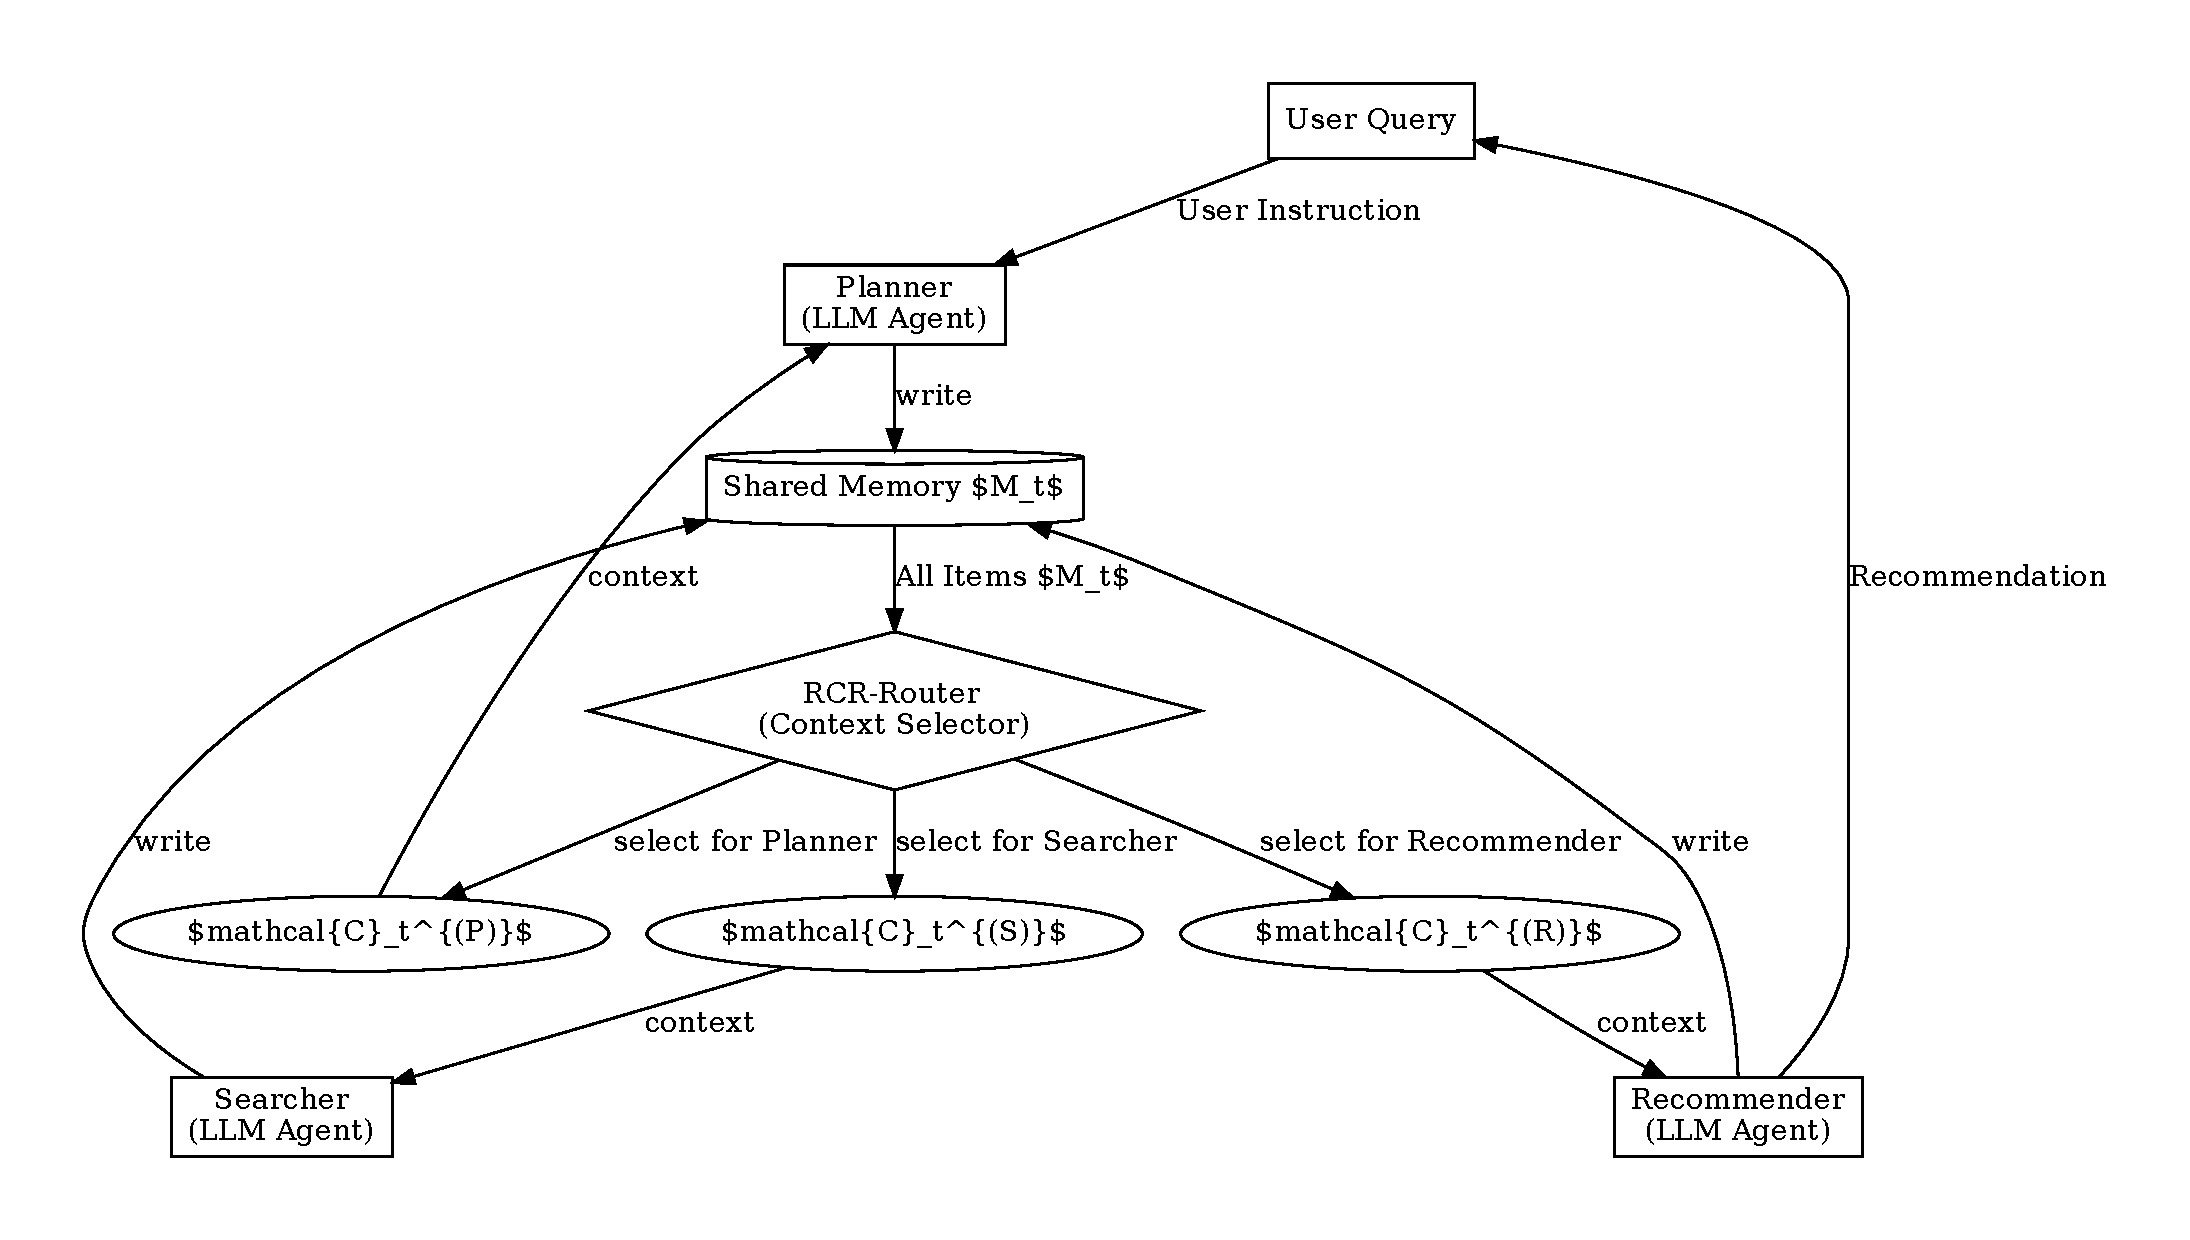
\includegraphics[width=1.0\linewidth]{fig/mcp_router_memory_flow.pdf}
    \caption{Memory flow diagram in RCR-Router. Each agent receives role-specific context slices from the shared memory $M_t$, processes them via an LLM, and appends new memory entries.}
    \label{fig:mcp_router_memory_flow}
\end{figure}

\begin{enumerate}
    \item \textbf{Memory Pool Initialization:} At time step $t$, the memory set $M_t$ consists of all past memory items $\{m_1, m_2, ..., m_t\}$ accumulated from prior agent outputs.
    
    \item \textbf{Token Budget Allocation:} For each agent role $i$, a pre-defined token budget $B_i$ is allocated (e.g., Planner: 1500 tokens, Searcher: 1000 tokens, Recommender: 800 tokens).
    
    \item \textbf{Memory Scoring:} Each memory item $m_j \in M_t$ is scored using an importance scorer $s(m_j, i, \text{stage}, t)$, where the score reflects the relevance of $m_j$ for agent $i$ at the current stage.
    
    \item \textbf{Semantic Filtering:} All memory items are ranked by their scores, and top-ranked items are greedily selected under the token constraint $B_i$, forming the contextual input $C_{t}^{(i)}$ for agent $i$.
    
    \item \textbf{Prompt Construction and Agent Invocation:} The filtered memory $C_{t}^{(i)}$ is converted into context text and inserted into the prompt template for the specific agent role, which is then passed to the LLM to generate the next action.
\end{enumerate}
\paragraph{Memory Update Strategy}
After each round of agent execution, RCR-Router:
\begin{enumerate}
    \item Selects a role-specific subset of $M_t$ based on predefined filters.
    \item Forms a prompt to query the LLM (or environment).
    \item Appends the resulting output as a new memory entry with timestamp and tags.
\end{enumerate}

\paragraph{Key Design Insight}
This staged memory routing allows each agent to operate within its own contextual window while contributing to a globally consistent shared memory. The design balances modularity and coherence, enabling flexible and interpretable agent collaboration for multi-turn decision-making in e-commerce scenarios.


%%%%%Added by Fan%%%%%
\section{C \quad Theoretical Analysis} \label{app:theorem} 

To formally ground our proposed RCR-Router architecture, we present a theoretical analysis of its core properties. We demonstrate that our design provides guarantees on resource efficiency and that the context routing mechanism can be framed as a well-understood optimization problem, justifying our use of an efficient heuristic. Finally, we prove that our iterative feedback loop leads to a progressive refinement of context quality over time.


\subsection{C.1 \quad Efficiency and Complexity}

\begin{comment}
\begin{definition}[Token Cost]
Let $\mathcal{T}(S)$ be the total token cost for a set of memory items $S$, defined as $\mathcal{T}(S) = \sum_{m \in S} \text{TokenLength}(m)$.
\end{definition}

\begin{theorem}[Guaranteed Token Efficiency]
\label{thm:efficiency}
For any agent $A_i$ at any interaction round $t$, the token cost of the context $C_t^i$ provided by RCR-Router is bounded by the total token cost of the shared memory $M_t$:
$$ \mathcal{T}(C_t^i) \le \mathcal{T}(M_t) $$
Furthermore, if the shared memory's cost exceeds the agent's budget, $\mathcal{T}(M_t) > B_i$, the token reduction is strictly positive:
$$ \mathcal{T}(C_t^i) < \mathcal{T}(M_t) $$
\end{theorem}

\begin{proof}
The proof follows from the definition of the routing mechanism.
\begin{enumerate}
    \item By definition of the routing mechanism (Algorithm 1) , the routed context is a subset of the shared memory, $C_t^i \subseteq M_t$. This implies $\mathcal{T}(C_t^i) \le \mathcal{T}(M_t)$.
    \item The routing mechanism explicitly enforces the token budget constraint $B_i$, ensuring that $\mathcal{T}(C_t^i) \le B_i$.
    \item Combining these, we have $\mathcal{T}(C_t^i) \le \min(\mathcal{T}(M_t), B_i)$, which directly proves the first part of the theorem.
    \item If $\mathcal{T}(M_t) > B_i$, then from step 2, $\mathcal{T}(C_t^i) \le B_i < \mathcal{T}(M_t)$, which proves the strict inequality.
\end{enumerate}
\end{proof}
\end{comment}

\begin{proposition}[NP-hardness of Optimal Context Routing]
\label{prop:nphard}
The problem of selecting a context $C' \subseteq M_t$ that maximizes the total importance score $\sum_{m \in C'} \alpha(m; R_i, S_t)$ subject to the token budget constraint $\mathcal{T}(C') \le B_i$, as formulated in Equation (1), is an instance of the 0/1 Knapsack Problem and is therefore NP-hard.
\end{proposition}

\begin{proof}
The problem maps directly to the 0/1 Knapsack Problem:
\begin{itemize}
    \item \textbf{Items:} The set of memory items $\{m_1, \dots, m_k\}$ in $M_t$.
    \item \textbf{Value of Item $j$:} The importance score, $v_j = \alpha(m_j; R_i, S_t)$.
    \item \textbf{Weight of Item $j$:} The token length, $w_j = \text{TokenLength}(m_j)$.
    \item \textbf{Knapsack Capacity:} The token budget, $W = B_i$.
\end{itemize}
The objective to maximize total value without exceeding capacity is the definition of the 0/1 Knapsack problem~\cite{karp2009reducibility}. Since 0/1 Knapsack is NP-hard, the optimal context routing problem is also NP-hard. This justifies the use of an efficient polynomial-time heuristic.
\end{proof}

\begin{theorem}[Optimality of the Importance-Greedy Heuristic]
\label{thm:greedy}
The greedy routing policy described in Algorithm 1 , which sorts memory items by their importance score $\alpha$ and adds them until the budget is met, finds the optimal solution to the context routing problem defined in Proposition~\ref{prop:nphard} if and only if all memory items $m \in M_t$ have a uniform token length.
\end{theorem}
\begin{proof}
This is a known result from combinatorial optimization. When all item weights ($\text{TokenLength}$) are uniform, the 0/1 Knapsack problem is solved optimally by a greedy strategy that sorts by value ($\alpha$) and selects the top items. Algorithm 1 implements exactly this strategy. If token lengths are non-uniform, this greedy approach is not guaranteed to be optimal.
\end{proof}

%\begin{comment}
\subsection{C.2 \quad Iterative Refinement and Convergence}

\begin{definition}[Context Quality]
\label{def:quality}
Let the quality of a context set $C$ for a future agent task, defined by role $R_k$ and stage $S_j$, be the average importance score of its constituent items: 
$$ Q(C | R_k, S_j) = \frac{1}{|C|} \sum_{m \in C} \alpha(m; R_k, S_j) $$
\end{definition}

\begin{lemma}[Monotonic Memory Relevance]
\label{lem:relevance}
Assume that the expected quality of an agent's structured output $O_t^i$ is a monotonically increasing function of the quality of its input context $C_t^i$. Given the Memory Update function (Equation 6) , which includes relevance filtering, the expected quality of the memory store at the next round, $E[Q(M_{t+1} | \cdot)]$, is non-decreasing with respect to the quality of the memory at the current round, $Q(M_t | \cdot)$.
\end{lemma}
\begin{proof}[Justification]
This lemma formalizes the "virtuous cycle" of the feedback loop. LLM agents are designed to produce relevant outputs from relevant contexts. The Memory Update mechanism  explicitly filters low-value outputs and integrates high-value ones, ensuring the memory pool is enriched over time.
\end{proof}

\begin{theorem}[Convergence of Iterative Context Refinement]
\label{thm:convergence}
Given Monotonic Memory Relevance (Lemma~\ref{lem:relevance}), the expected quality of the context $C_t^i$ routed to an agent $A_i$ is non-decreasing over interaction rounds $t$.
$$ E[Q(C_{t+1}^i | R_i, S_{t+1})] \ge E[Q(C_t^i | R_i, S_t)] $$
\end{theorem}
\begin{proof}
\begin{enumerate}
    \item From Lemma~\ref{lem:relevance}, the shared memory pool $M_{t+1}$ is expected to have a higher density of relevant items than $M_t$.
    \item The RCR-Router's selection mechanism (Algorithm 1) is designed to select the subset of items with the highest importance scores from the memory pool.
    \item Applying a selection function that chooses the "best" items to a "better" pool ($M_{t+1}$) will, in expectation, yield a selected subset ($C_{t+1}^i$) of higher quality than applying it to the previous pool ($M_t$).
    \item Therefore, the iterative feedback loop ensures a non-decreasing trajectory for the expected quality of the routed context, formalizing the concept of progressive refinement. This supports the empirical results of the iterative routing ablation study .
\end{enumerate}
\end{proof}
%\end{comment}


\section{D \quad  Extended Role Examples in Multi-Agent Systems}  \label{app:broader} 

We consider a \textbf{multi-agent LLM system} composed of $N$ collaborative agents $\mathcal{A} = \{ A_1, A_2, \dots, A_N \}$ interacting over a shared task. Each agent $A_i$ operates with a specific \textit{role} $R_i$ and engages in discrete \textit{interaction rounds} $t = 1, 2, \dots, T$, collaborating with other agents and external tools.

Typical roles include \textit{planner}, \textit{executor}, and \textit{summarizer}; however, our framework supports a broader set of roles to address diverse task requirements. For example:
\begin{itemize}
    \item \textbf{Retriever}: fetches and verifies external knowledge from retrieval systems;
    \item \textbf{Verifier}: assesses factual consistency and detects reasoning errors;
    \item \textbf{Critic}: reviews intermediate steps and suggests revisions;
    \item \textbf{Rewriter}: paraphrases or refines outputs for clarity or style;
    \item \textbf{Refiner}: improves partial solutions based on feedback or tool outputs.
\end{itemize}

This flexibility enables role specialization and division of labor, which is key to efficient and accurate multi-agent coordination.

At each round $t$, agents exchange messages and perform reasoning based on a \textbf{Shared Memory Store} $M_t$, which contains:
\begin{itemize}
    \item \textbf{Agent interaction history}: prior communication between agents;
    \item \textbf{Task-relevant knowledge}: external facts, retrieved documents, or tool outputs;
    \item \textbf{Structured state representations}: entities, plans, and tool traces encoded in structured formats (YAML, graphs, tables).
\end{itemize}

\section{E \quad Details of Importance Scorer}
\label{appendix:importance_scorer}

The \textbf{Importance Scorer} used in the RCR-router is designed to estimate the utility of each memory item $m \in M_t$ for a specific agent $A_i$ at interaction time $t$, given its role $R_i$ and task stage $S_t$. To keep routing efficient and interpretable, we adopt a lightweight heuristic-based scoring mechanism, which combines the following three components:

\begin{itemize}
    \item \textbf{Role Relevance.}  
    Each agent is assigned a semantic role (e.g., Planner, Executor, Summarizer). We maintain a role-specific keyword list $\mathcal{K}_i$ for each role $R_i$, manually curated from the task schema. A memory item $m$ is scored higher if it contains any keywords from $\mathcal{K}_i$. Formally:
    $$
    \text{Score}_{\text{role}}(m) = \mathbb{1}[\exists k \in \mathcal{K}_i \text{ such that } k \in m]
    $$

    \item \textbf{Task Stage Priority.}  
    Certain memory items are more relevant to specific task stages (e.g., context planning, candidate filtering, final decision). For each stage $S_t$, we define a preferred item type (e.g., query history, tool results, prior plans). We assign higher scores to items matching the preferred type for the current stage. Let $\mathcal{T}_t$ be the set of relevant memory types at stage $S_t$:
    $$
    \text{Score}_{\text{stage}}(m) = \mathbb{1}[\text{Type}(m) \in \mathcal{T}_t]
    $$

    \item \textbf{Recency.}  
    Memory items generated more recently (i.e., closer to $t$) are typically more relevant. We compute recency score based on their relative position in the memory buffer, using a decaying weight:
    $$
    \text{Score}_{\text{recency}}(m) = \exp(-\lambda \cdot (t - t_m))
    $$
    where $t_m$ is the timestamp or round index when $m$ was created, and $\lambda$ is a tunable decay factor.
\end{itemize}

The final importance score is computed as a weighted combination:
$$
\alpha(m; R_i, S_t) = w_1 \cdot \text{Score}_{\text{role}}(m) + w_2 \cdot \text{Score}_{\text{stage}}(m) + w_3 \cdot \text{Score}_{\text{recency}}(m)
$$
where $w_1, w_2, w_3$ are hyperparameters (e.g., set to 1.0 by default).

This design balances interpretability, extensibility, and efficiency, and allows plug-in of learned components if desired.

\section{F \quad  Modular Multi-Agent System Design for ALFWorld}
ALFWorld~\cite{ALFWorld20} is an embodied instruction-following environment where agents must complete household tasks through navigation and object manipulation.

We define a structured multi-agent framework for ALFWorld, where each agent specializes in a specific sub-task and interacts via a shared memory interface. This architecture supports effective division of labor and token-efficient context routing.

\begin{table}[h]
\centering
\caption{Agent Roles in ALFWorld for RCR-Router}
\label{tab:alfworld_roles_detailed}
\begin{tabular}{l|p{11.2cm}}
\toprule
\textbf{Agent Role} & \textbf{Description} \\
\midrule
\textbf{Planner} &
\begin{itemize}
  \item Parses natural language task instructions.
  \item Decomposes them into symbolic subgoals (e.g., \texttt{Find(bottle)}).
  \item Integrates feedback from memory and updates plan iteratively.
\end{itemize}
\\
\hline
\textbf{Searcher / Navigator} &
\begin{itemize}
  \item Explores the simulated environment to discover goal-relevant objects.
  \item Navigates the agent to specified locations using spatial reasoning.
  \item Supports multi-hop search via memory-informed object-location mapping.
\end{itemize}
\\
\hline
\textbf{Interactor} &
\begin{itemize}
  \item Performs object-level actions (e.g., \texttt{Pickup}, \texttt{PutIn}, \texttt{Open}).
  \item Executes low-level manipulations in response to subgoal execution.
  \item Verifies interaction success and provides outcomes to shared memory.
\end{itemize}
\\
\bottomrule
\end{tabular}
\end{table}





\vspace{2mm}

\noindent The agents communicate via a shared semantic memory store $\mathcal{M}_t$, with memory slices dynamically routed at each timestep $t$ using a token-budgeted context router (e.g., RCR-Router). Each agent $A_i$ receives a context $C_t^i \subseteq \mathcal{M}_t$ based on its \textit{role} and \textit{task stage}.

\subsubsection*{Interfaces and Coordination}

\subsubsection*{Agent Interfaces and Inputs}

\begin{itemize}
    \item \textbf{Planner Input:} Natural language task instruction.
    \item \textbf{Planner Output:} High-level sub-goals $\mathcal{P} = [g_1, g_2, \dots, g_k]$.
    \item \textbf{Searcher Input:} Sub-goal type + prior memory state; queries environment for candidate object locations.
    \item \textbf{Navigator Input:} Sub-goal location + current agent position.
    \item \textbf{Interactor Input:} Goal object/location + interaction command (\texttt{Pickup}, \texttt{Open}, etc.).
    \item \textbf{Memory Access:} All agents interact with shared memory $\mathcal{M}_t$ using read/write APIs, managed by RCR-router.
\end{itemize}

\subsubsection*{Execution Flow }

\begin{enumerate}
    \item \textbf{Planner} interprets the instruction and generates sub-goals.
    \item \textbf{Searcher} queries the environment (via \textbf{Perception}) to identify objects satisfying current sub-goal.
    \item \textbf{Navigator} moves the agent toward target objects or locations.
    \item \textbf{Interactor} performs the necessary environment interaction.
    %\item \textbf{Memory Agent (RCR-router)} dynamically routes relevant memory slices to agents and updates $\mathcal{M}_{t+1}$.
    \item \textbf{Evaluator} verifies task completion and optionally signals \textbf{Planner} for replanning.
\end{enumerate}

\subsubsection*{Design Benefits}

\begin{comment}
    

\begin{itemize}
    \item \textbf{Role Modularity:} Each agent role is decoupled, enabling independent development and testing.
    \item \textbf{Semantic Routing:} The RCR-router delivers role-aware, context-efficient memory slices under token constraints.
    \item \textbf{Iterative Feedback:} Memory updates at each round support dynamic adjustment and coordination.
    \item \textbf{Scalable Design:} The framework accommodates additional roles (e.g., Reasoner, Explainer) without architectural change.
\end{itemize}
\end{comment}

%\subsubsection*{Design Benefits of Modular Multi-Agent System for ALFWorld}

\begin{itemize}
    \item \textbf{Role Modularity and Separation of Concerns:}
    Each agent is assigned a distinct functional role—such as planning, navigation, or interaction—enabling clean abstraction of responsibilities. This separation simplifies debugging, benchmarking, and targeted model improvements.

    \item \textbf{Token-Efficient Context Routing:}
    The integration of RCR-router ensures that each agent receives only task-relevant memory slices filtered by semantic importance, role identity, and token budget. This significantly reduces redundant communication and enhances inference efficiency.

    \item \textbf{Structured Execution with Iterative Feedback:}
    Agents operate in a recurrent loop, reading from and writing to a centralized memory store $\mathcal{M}_t$. This allows for dynamic plan revisions, success verification, and coordination between planning and execution modules.

    \item \textbf{Perceptual Grounding and Semantic Sharing:}
    Agents share a structured memory that encodes grounded observations (e.g., object types, spatial positions, interaction outcomes), facilitating semantic consistency and spatial reasoning across modules.

    \item \textbf{Scalability and Extensibility:}
    The architecture accommodates additional roles such as \texttt{Reasoner}, \texttt{Memory Summarizer}, or \texttt{Language Explainer} without changes to the routing pipeline. It generalizes across different task settings in embodied environments.

    \item \textbf{Backend Compatibility and Reusability:}
    Each agent can be instantiated using different backbone LLMs or decision models (e.g., DeepSeek, GPT-4, distilled variants), supporting plug-and-play experimentation without modifying upstream pipeline logic.
\end{itemize}


\paragraph{Evaluation on ALFWorld.}
Table~\ref{tab:alfworld_results} reports the overall performance comparison on the ALFWorld benchmark under a fixed per-agent token budget of $B_i = 2048$. We evaluate three routing strategies: \textit{Full-Context}, \textit{Static Routing}, and our proposed \textit{RCR-router}. RCR-router achieves the best performance across all metrics. Specifically, it reduces the average runtime from 145.3s (Full-Context) and 122.8s (Static) to 96.4s, while also lowering token usage to 4.39K—representing a 35.6\% reduction over Full-Context. 

In terms of answer quality, RCR-router attains a score of 4.42, significantly higher than both baselines (3.91 and 4.07). Standard QA metrics also improve: RCR-router achieves 66.7\% precision, 67.9\% recall, and 67.3\% F1, compared to 58.2/60.1/59.1 for Full-Context and 61.5/63.0/62.2 for Static Routing. These results confirm that our method improves both efficiency and accuracy in multi-agent embodied environments.

\begin{table*}[t]
\centering
\caption{Overall Performance Summary across Benchmarks (with per-agent token budget $B_i = 2048$). We report runtime, token usage, LLM-based Answer Quality, and standard QA metrics. RCR-router outperforms baselines in both efficiency and accuracy.}
\label{tab:alfworld_results}
\begin{tabular}{c|c|c|c|c|c|c|c}
\toprule
\multirow{2}{*}{\textbf{Benchmark}} & \multirow{2}{*}{\textbf{Method}} & \multicolumn{6}{c}{\textbf{Results}} \\
\cline{3-8}
& & Avg Runtime (s) & Token (K) & Answer Quality & Precision & Recall & F1 \\
\midrule
\multirow{3}{*}{ALFWorld} 
& Full-Context    & 145.3 & 6.82 & 3.91 & 58.2 & 60.1 & 59.1 \\
& Static Routing  & 122.8 & 5.12 & 4.07 & 61.5 & 63.0 & 62.2 \\
& RCR-router      &  96.4 & 4.39 & \textbf{4.42} & \textbf{66.7} & \textbf{67.9} & \textbf{67.3} \\
\bottomrule
\end{tabular}
\end{table*}


\section*{G \quad  Modular for Multi-Agent System Design in WebShop}
%\section*{Roles in WebShop Multi-Agent System}
WebShop~\cite{yao2022webshop} is a text-based e-commerce environment where agents must fulfill shopping goals through search, click, and buy tool invocations.

We define the following modular roles for WebShop agent collaboration:

\begin{itemize}
    \item \textbf{Planner (Query Decomposer)}:
    \begin{itemize}
        \item Interprets the user's natural language instruction and extracts structured constraints.
        \item Identifies product attributes (e.g., size, color, category, quality keywords).
        \item Constructs a canonical query or subgoals to guide retrieval.
    \end{itemize}

    \item \textbf{Searcher (Retriever)}:
    \begin{itemize}
        \item Uses the structured query from the Planner to search a product corpus (e.g., via Pyserini or ScraperAPI).
        \item Retrieves top-$k$ relevant product candidates.
        \item May refine results using user-specific filters or historical memory.
    \end{itemize}

    \item \textbf{Recommender (Evaluator)}:
    \begin{itemize}
        \item Analyzes product candidates returned by the Searcher.
        \item Matches them against instruction attributes (both explicit and implicit).
        \item Selects and ranks products and generates a natural language justification or recommendation.
    \end{itemize}
\end{itemize}

We design a modular multi-agent system for WebShop consisting of three specialized roles:

\begin{table}[t]
\centering
\caption{Agent Roles and Responsibilities in WebShop Multi-Agent System}
\label{tab:webshop_roles}
\begin{tabular}{l|p{10.5cm}}
\toprule
\textbf{Agent Role} & \textbf{Responsibilities} \\
\midrule
\textbf{Planner} & 
\begin{itemize}
    \item Parses user instructions (e.g., ``I need a high-quality storage case for my Infinitipro'').
    \item Extracts key attributes: category, brand, size, quality, etc.
    \item Generates structured queries or sub-goals for the Searcher.
\end{itemize} \\
\hline
\textbf{Searcher} & 
\begin{itemize}
    \item Retrieves relevant products using structured queries and a product index (e.g., Pyserini).
    \item Ranks results based on semantic similarity and attribute match.
    \item Refines query based on contextual or memory feedback.
\end{itemize} \\
\hline
\textbf{Recommender} & 
\begin{itemize}
    \item Evaluates product candidates against user preferences and soft constraints.
    \item Filters or re-ranks items based on implicit signals (e.g., ``GMO-free'').
    \item Generates natural language justifications and final suggestions.
\end{itemize} \\
\bottomrule
\end{tabular}
\end{table}





\subsubsection*{Execution Flow }

Given a user instruction, our WebShop multi-agent system proceeds as follows:

\begin{enumerate}
    \item \textbf{Planner} receives the instruction and performs constraint extraction (e.g., attributes, options), forming a structured query.
    
    \item \textbf{Searcher} takes the query and retrieves candidate products using a retrieval engine (e.g., Pyserini + indexed corpus, or live ScraperAPI).
    
    \item \textbf{Recommender} evaluates the retrieved products, matching them against user constraints and preferences, and generates a ranked shortlist with textual rationales.
    
    \item \textbf{(Optional)} The final product or product list is returned to the user, or used to simulate downstream actions (e.g., “choose [Product Title]”, “choose [Option]”, etc.).
\end{enumerate}

Agents interact via a shared structured memory $M_t$, with context routed at each iteration based on role and task stage.

\begin{table*}[t]
\centering
\caption{Overall Performance Summary on WebShop Benchmark (with per-agent token budget $B_i = 2048$). We report runtime, token usage, LLM-based Answer Quality, and standard QA metrics. RCR-router achieves superior efficiency and recommendation quality.}
\label{tab:webshop_results}
\begin{tabular}{c|c|c|c|c|c|c|c}
\toprule
\multirow{2}{*}{\textbf{Benchmark}} & \multirow{2}{*}{\textbf{Method}} & \multicolumn{6}{c}{\textbf{Results}} \\
\cline{3-8}
& & Avg Runtime (s) & Token (K) & Answer Quality & Precision & Recall & F1 \\
\midrule
\multirow{3}{*}{WebShop} 
& Full-Context    & 180.2 & 9.78 & 3.85 & 55.4 & 57.6 & 56.5 \\
& Static Routing  & 142.6 & 7.12 & 4.01 & 60.7 & 62.5 & 61.6 \\
& RCR-router      & 110.9 & 6.03 & \textbf{4.36} & \textbf{64.8} & \textbf{65.9} & \textbf{65.3} \\
\bottomrule
\end{tabular}
\end{table*}

\subsubsection*{Design Benefits}
\begin{itemize}
\item \textbf{Scalability:} The architecture supports the inclusion of additional specialized roles (e.g., Critic, Explainer, Dialogue Handler) without modifying the core system, allowing for progressive enhancement of capabilities.

\item \textbf{Context-Aware Interaction:} Through memory abstraction and structured routing, agents can share and retrieve relevant semantic information, enhancing coordination and reducing context redundancy.

\item \textbf{Token Efficiency:} Leveraging selective routing (e.g., via RCR-Router), agents only receive context slices pertinent to their role and current task state, minimizing unnecessary token usage under LLM constraints.

\item \textbf{Backend-Agnostic Compatibility:} The modular design is compatible with diverse LLM backends (e.g., OpenAI, DeepSeek, ChatGLM), as long as agents operate under a consistent prompt-response protocol.

\item \textbf{Interpretable Reasoning:} Role-specific outputs (e.g., structured plans, ranked product lists, natural language recommendations) improve system interpretability and facilitate human-in-the-loop evaluation.
\end{itemize}

\paragraph{Evaluation on WebShop.}
We evaluate our method on the WebShop benchmark, a realistic multi-agent shopping assistant task involving semantic retrieval, attribute grounding, and decision recommendation. As shown in Table~\ref{tab:webshop_results}, our proposed RCR-router achieves the best overall performance across all evaluation metrics. Specifically, it reduces average runtime by 22\% compared to Static Routing and by 38\% compared to the Full-Context baseline. It also achieves the lowest token consumption (6.03K) while improving answer quality to 4.36. Moreover, RCR-router significantly outperforms other methods in standard QA metrics, achieving an F1 score of 65.3, representing a +3.7 improvement over Static Routing and a +8.8 gain over Full-Context. These results highlight the effectiveness of our role- and stage-aware context routing framework in reducing overhead and enhancing decision accuracy in complex multi-agent interactions.

\begin{comment}
    

\section{F \quad Illustrative Example of Multi-Role Collaboration}

To illustrate the effectiveness of our multi-agent setup, we present an example of how different roles collaborate to solve a HopOotQa QA task:

\paragraph{User Query:} \textit{Who is the spouse of the Green performer?}

\begin{enumerate}
    \item \textbf{Planner} ($A_1$) analyzes the query and decomposes it into subgoals:
    \begin{itemize}
        \item Identify the entity referred to as the "Green performer".
        \item Find the spouse of that entity.
    \end{itemize}

    \item \textbf{Retriever} ($A_2$) issues two document retrieval queries based on the planner’s subgoals:
    \begin{itemize}
        \item ``Green + performer'' → returns a document stating \textit{Green is an album by Steve Hillage}.
        \item ``Steve Hillage + spouse'' → retrieves a document identifying \textit{Miquette Giraudy as Hillage’s partner}.
    \end{itemize}

    \item \textbf{Executor} ($A_3$) integrates retrieved knowledge and produces the intermediate answer:
    \begin{quote}
        ``The Green performer is Steve Hillage, and his spouse is Miquette Giraudy.''
    \end{quote}

    \item \textbf{Verifier} ($A_4$) cross-checks retrieved facts and entity disambiguation to ensure logical consistency. It confirms that the inference chain is valid.

    \item \textbf{Rewriter} ($A_5$) refines the final answer for clarity and style:
    \begin{quote}
        ``Miquette Giraudy is the spouse of Steve Hillage, the performer associated with the album \textit{Green}.''
    \end{quote}
\end{enumerate}

This modular pipeline showcases the benefits of role-aware routing and structured memory, allowing each agent to focus on a well-defined function while collectively producing a high-quality, explainable answer.

\end{comment}
